\section{A language for specifying AO design rules}
\label{sec:drlang}

%XXX CRIAR FIGURA COM O META-MODELO S� COM O LADO ESQUERDO E COLOCAR NO DIRETORIO
%XXX Incluir a nova BNF?
%XXX Criterios de matching
%XXX Implementacao atual usando ABC
%XXX Discutir a implementacao explicita da interface por ambos

In this section we present the \emph{Language for Specifying
Design Rules (LSD)}. The main objective of this language is to
decouple syntactically and semantically classes and aspects,
maximizing independent development opportunities. Through the
definition of Design Rules we argue that both class and aspect
developers can work independently if a minimum set of constraints
is defined and respected.

LSD was defined as a way of expressing clearly and unambiguously
design rules established during all development phases, specially
during software design. The language serves as a mechanism for
creating more modular software, because it decouples classes and
aspects through the establishment of the minimum requirements to
their parallel development.

The initial motivation for the language development was improving
modularity of aspect-oriented systems. However, other design
rules, like those defined during architectural design, can be
naturally expressed by the language.

On the other hand, its utilization requires the creation of new
artifacts to contain design rule specifications. Also, in order to
define appropriate design rules its expected that software
designers have enough experience for that. Additionally,
developers must get used to new language constructs. In spite of
that, explicitly expressing the design rules, and specially being
capable of verifying them, makes easy the task of developing new
components.

In this section we present LSD main constructs, based on previous
work... %~cite\{DoseaLAWASP}.

\subsection{LSD overview}
\label{sec:lsdoverview}

%---------------------------------------------

Many Object-Oriented programming languages provide the concept of
interface which specify a public set of methods and constants
obligatorily provided by any class that declares to implement it.
This interface notion allows developers to create separated and
narrow interfaces to different clients of the same class, limiting
the coupling between them.

Our concept of interface, which we call a \emph{Design Rule}, is
wider. A Design Rule contains a set of constraints that must be
followed by components that declare to implement them. These
constraints are automatically verified by a tool that points out
when some constraint is disrespected by class and aspect
developers.

Figure~\ref{fig:meta-model} shows the Design Rules specification
language meta-model. A rule description is composed by one or more
structural rules (section~\ref{sec:structuralrules}). They are
used to define structural constraints for classes and aspects.
Thus, a class can define fields, method signatures and behavioral
rules. These behavioral rules (section~\ref{sec:behavioralrules})
can be defined within classes and aspects scope or within their
methods and advices (only aspects).

\begin{figure}[htp]
  \begin{center}
  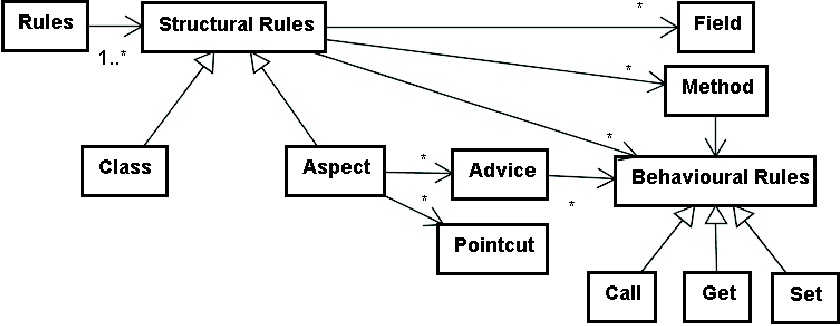
\includegraphics[width=1.0\textwidth]{images/meta-model}\\
  \caption{Design Rule Language and Configuration Module Meta-Models}
  \label{fig:meta-model}
  \end{center}
\end{figure}

\subsection{Structural Rules}
\label{sec:structuralrules}

Structural Rules are design rules that describe constraints about
members of classes and aspects. Their format is similar to the
interface description in Java~\cite{JAVA}, but it is possible to
include additional constraints (beyond required public methods and
constants), like attributes that must be declared and required
method visibility. Besides, there are specific constraints about
aspects structure, like requiring an specific pointcut declaration
and/or advice.

Listing~\ref{lst:dr1} shows examples of structural rule
descriptions to be respected by classes and aspects. Line 1
contains the declaration of the \texttt{System} design rule that
aggregates a set of \emph{structural rules}. Following, it appears
the \emph{structural rule} declaration for
\texttt{ComponentRecord} to be respected by classes. It requires
the declaration of two methods with compatible signatures (Lines
2-5). There is also the \texttt{Component} \emph{structural rule}
(Lines 6-8), which must be respected by classes. The last
\emph{structural rule} declared (Lines 9-16), called
\texttt{TransactionalManagement} must be followed by aspects,
which must contain a pointcut \texttt{service} and the
\emph{advices before} and \emph{around} to this pointcut.

\scriptsize
\begin{lstlisting}[frame=single, caption={Structural Rule for Transaction Management.},label=lst:dr1,
                numbers=left,
                language=Java,
                morekeywords={dr, aspect, pointcut}]
dr System {
    class ComponentRecord {
        public void insert(Component c);
        public void delete(Component c);
    }
    class Component {
        int key;
    }
    aspect TransactionalManagement {
      pointcut service(): execution(ComponentRecord.insert(Component)) ||
                          execution(ComponentRecord.delete(Component));
      before(): service() {
      }
      after(): service() {
      }
    }
}
\end{lstlisting} \normalsize


\texttt{System} design rule declares the minimum requirements so
that components \texttt{ComponentRecord}, \texttt{Component} and
\texttt{TransactionalManagement} can be developed in parallel. So,
for example, the \texttt{ComponentRecord} developer needs to know
only that it must implement methods \texttt{insert} and
\texttt{delete} so that other components works correctly. The
language enables the specification of \emph{structural rules} to
attribute declaration, useful in cases that clients of the
component requiring it. An example of it appears in
Listing~\ref{lst:dr1} within the \texttt{Component}
\emph{structural rule}. It requires that Component classes provide
an \texttt{attribute} int called \texttt{key}.


\subsection{Behavioral Rules}
\label{sec:behavioralrules}

A \emph{behavioral rule} provides a mechanism for specifying
constraints about the behavior of components. When a behavioral
rule is defined within the scope of a class or aspect it means
that it has to be respected at any place, for example, if a rule
\emph{call} is used within the scope of a class, it means that the
required method must be called at least once in this class.
Another example is requiring a read (or write) of an specific
attribute within a certain scope.

The Table~\ref{tbl:commands} shows the \emph{behavioral rules}
provided by the language. The scope of these rules includes
classes, aspects, methods and advices. Every rule initiated by 'x'
guarantees that the rule will be followed only in the defined
scope and this will not be possible in any other location. For
example, the \emph{xcall} rule guarantees that an specific method
will be called exclusively within the scope in which it was
defined. Calls outside the scope are not allowed. In case that the
rule \emph{xcall(method)} exists in more than one scope for the
same method, then this call can only occur within these defined
scopes.

\begin{table}
  \centering
  \caption{Behavioral Rules provided by the LSD.}\label{tbl:commands}
    \begin{tabular}{|c|p{10.5cm}|}
      \hline
      \textbf{Rule} & \textbf{Description}\\
      \hline
      \emph{call(method)} & It must have a call to the method passed as parameter within the defined scope.\\
      \hline
      \emph{xcall(method)} & It must have a call to the method passed as parameter exclusively in the defined scope.\\
      \hline
      \emph{set(attribute)} & It must have an state change on the attribute passed as parameter within the defined scope.\\
      \hline
      \emph{xset(attribute)} & It must have an state change on the attribute passed as parameter exclusively within the defined scope.\\
      \hline
      \emph{get(attribute)} & It must have an state access to the attribute passed as parameter within the defined scope.\\
      \hline
      \emph{xget(attribute)} & It must have an state access to the attribute passed as parameter exclusively within the defined scope.\\
      \hline
    \end{tabular}
\end{table}

These rules are also useful to guarantee, for example, that a
method must not be called in a given scope, by using the negation
operator (!). When a \emph{behavioral rule} is defined within the
scope of a class or aspect, it is valid for the entire class. One
\emph{call} within a class indicates that at some point of the
class that call must occur.

\scriptsize
\begin{lstlisting}[frame=single, caption={Behavioral Rules for Transaction Management.},
                   label=lst:dr2, numbers=left, language=Java,
                   morekeywords={dr, xcall, aspect, pointcut} ]
dr System {
    class ComponentRecord {
        public void insert(Component c);
        public void delete(Component c);
    }
    class Component {
        int key;
    }
    class Persistence {
        void beginTransaction();
        void endTransaction();
        void openConnection();
        void closeConnection();
    }
    aspect TransactionalManagement {
      pointcut service(): execution(ComponentRecord.insert(Component));
      before(): service() {
          xcall( Persistence.beginTransactional() );
      }
      after(): service() {
          xcall( Persistence.endTransactional() );
      }
   }
}
\end{lstlisting} \normalsize

Listing~\ref{lst:dr2} shows the using of the \emph{xcall
behavioral rule} (Lines 18 and 21). These two rules indicate that
methods must be called exclusively within the advice scope,
prohibiting calls from any other place among the components
specified by the design rule \texttt{System}. For example, if the
method \texttt{Persistence.beginTransaction()} was called from the
\texttt{delete} method of the class that implement the
\texttt{ComponentRecord} \emph{structural rule} an error would be
presented to the user. Thus, through simple rules it is possible
to improve system modularity, documenting the interaction rules
between components and guaranteing that they are being followed by
using a verifier. It is important that classes and aspects always
implement the \emph{design rules} documented by the software
designer. If this is not done, it is impossible to guarantee that
they will be respected. For example, a class that implements no
\emph{structural rules} defined by the \texttt{System}
\emph{design rule} can call the method
\texttt{Persistence.beginTransaction()}, even if in the
architecture project this call should only occur within the aspect
responsible for transaction management.

%-------------------------------

\subsection{Explicit implementation of Design Rules}
\label{sec:explicitimpldr}

Trying to keep similarity with Java interfaces concept, and
following the LSD principle of establish an interface between
classes and aspects, LSD requires that both class and aspect
explicitly implements the design rules.

In order to developers being aware of the design rules they must
respect, the components being developed must include the name of
all design rules that it implements in the \emph{implements
clause} like classes that implement ordinary interfaces.
Additionally, for each implemented design rule, it must be provide
the name of one or more the structural rules.

Thus, if the class developer needs to make a change, it is easier
to identify which design rules must be respected, facilitating
evolution some jobs and preventing some errors. Besides, its use
enables automatic verification and separate compilation. The using
of \emph{implements} obligates a class or aspect to follow all the
rules defined by the corresponding \emph{structural rule}.

\scriptsize
\begin{lstlisting}[frame=single, caption={Explicit implementation of the Design Rule System.},
                   label=lst:comp1,
                   numbers=left, language=Java,
                   morekeywords={dr, xcall, aspect, pointcut}]
class UserRecord implements System(ComponentRecord) {
    ...
}

class User implements System(Component) {
    ...
}

class Persistence implements System(Persistence) {
    ...
}

aspect TransactionalManagement implements
System(TransactionalManagement) {
    ...
}
\end{lstlisting} \normalsize

Listing~\ref{lst:comp1} shows examples of components that follows
the \emph{design rule} \texttt{System}. For example, classes
\texttt{UserRecord} (Lines 1-3), \texttt{User} (Lines 5-7) and
 \texttt{Persistence} (Lines 9-11) indicate the names of their corresponding \emph{structural rules},
\texttt{ComponentRecord}, \texttt{Component} and
\\texttt{Persistence}, respectively. In an identical form, aspect
\texttt{TransactionalManagement} (Lines 13-16) implements
\texttt{System} and the corresponding \emph{structural rule}
\texttt{TransactionalManagement}.


\subsection{Additional constraints}
\label{sec:additionalconstraints}

Previous sections discussed the general idea of the LSD. In this
section we present more language constructs that provide ways of
expressing additional constraints.

\subsubsection{Modifiers}

The first one of them is related to components modifiers. It might
be necessary that a certain class, for example, have public and
not package visibility.

Listing~\ref{lst:drmodifiers} shows part of the design rule
\texttt{System}. \texttt{ComponentRecord} requires that classes
that implement the design rule \texttt{System} are \texttt{public}
classes and provide two \texttt{public} methods with a
\texttt{void} return type and with a parameter \texttt{Component}.
Others modifiers are accepted, like \texttt{final},
\texttt{synchronized} and \texttt{abstract}, since the language is
focused on specifying the minimum requisites about the component
structure.

\scriptsize
\begin{lstlisting}[frame=single, caption={Modifiers constraints.},
                   label=lst:drmodifiers, numbers=left, language=Java,
                   morekeywords={dr, xcall, aspect, pointcut} ]
dr System {
    public class ComponentRecord {
        public void insert(Component c);
        public void delete(Component c);
    }
    public class Component {
        private int key;
    }
    ...
}
\end{lstlisting} \normalsize

Additionally, listing~\ref{lst:drmod} contains a
\texttt{Component} class that must be \texttt{public}. Also, it
must provide a \texttt{private} attribute called \texttt{key} of
\texttt{int} type. It might be strange to define a constraint
about a private part of a class, but sometimes aspects need to
refer to private parts of classes. If this dependency is defined
in a design rule, it is possible to explicitly express it.

\subsubsection{Implements/Extends}

Another interesting type of constraint is to require that the
class implementing a certain \emph{structural rule} implements or
extends an specific type.

An example of this constraint is shown in
Listing~\ref{lst:drimpext}. Classes that implement the structural
rule \texttt{ComponentRecord} must explicitly implement the
interface \texttt{BaseRecord}. Following, the structural rule
\texttt{Component} must extend directly class
\texttt{BaseComponent}.

\scriptsize
\begin{lstlisting}[frame=single, caption={Implements/Extends constraints.},
                   label=lst:drimpext, numbers=left, language=Java,
                   morekeywords={dr, xcall, aspect, pointcut} ]
dr System {
    public class ComponentRecord implements BaseRecord {
        public void insert(Component c);
        public void delete(Component c);
    }
    public class Component extends BaseComponent {
        private int key;
    }
    ...
}
\end{lstlisting} \normalsize


\subsubsection{Inter-type declarations}

Inter-type declarations enable aspects to introduce attributes and
methods in classes. At the same time that it is an interesting
mechanism, it may create dependencies between classes and aspects.
This mechanism is frequently used in aspect-oriented software
product lines to introduce variable method implementations or
attributes values in classes. Design rules can be used to
explicitly create a contract between classes and aspects
introducing the variabilities.

Listing~\ref{lst:dritd} shows a design rule
\texttt{ScreenAtributtes} that declares two structural rules:
\texttt{MainScreen} and \texttt{SizeVariability}. The last one
must provide two inter-type declarations of fields \texttt{WIDTH}
and \texttt{HEIGHT} in the class that implement the structural
rule \texttt{MainScreen}. As a consequence, the class developer
can be sure that these two attributes will exist and can use it.

\scriptsize
\begin{lstlisting}[frame=single, caption={Implements/Extends constraints.},
                   label=lst:dritd, numbers=left, language=Java,
                   morekeywords={dr, xcall, aspect, pointcut} ]
dr ScreenAttributes {
    class MainScreen {
       ...
    }
    aspect SizeVariability {
        public static final int MainScreen.WIDTH;
        public static final int MainScreen.HEIGHT;
    }
}
\end{lstlisting} \normalsize

\subsection{Summary of constraints}
\label{sec:summaryofconstraints}

%-------------------------------
\subsubsection{Covered constraint types}

Covered Constraint Types

Required/Prohibited

Classes, Interfaces, Aspects

Fields, Methods, ITD, Advices, Pointcuts

Inheritance / Interface implementation

Method Calls

Attribute Get / Set


\subsubsection{Uncovered but planned constraint types}

Exceptions

Member Expressions

Class/Interface/Aspect Expressions

\subsection{LSD implementation}

LSD has an initial implementation using the ABC extensible
compiler for AspectJ~\ref{ABC}.

Descrever o ABC.

Descrever como o ABC foi estendido

Mostrar uma figura com o funcionamento logico do verificador.

Descrever alguma experiencia sobre a facilidade de extensao (ou
nao) do abc.

%XXX Implementacao atual usando


%---------------------------------------------
% PARTE DE ARTIGO ANTIGO


%In this section we present a Design Rule specification language.
%The main objective of this language is to decouple syntactically
%and semantically classes and aspects, maximizing independent
%development opportunities. Through the definition of Design Rules
%we argue that both class and aspect developers can work
%independently if a minimum set of constraints is defined and
%respected.
%
%\scriptsize
%\begin{lstlisting}[frame=single,
%                   caption={Display Update Design Rule.},
%                   label=lst:displayUpdateDR,
%                   numbers=left,
%                   language=Java,
%                   morekeywords={dr, xcall}]
%dr DRUpdateShape {
%    interface IShape {
%        void moveBy(int dx, int dy);
%    }
%
%    class Shape implements IShape {
%        void moveBy(int dx, int dy) {
%          xset(IShape+.*);
%        }
%    }
%
%    class Display {
%        void update();
%    }
%
%    aspect UpdateSignaling {
%        pointcut change():
%            execution( void IShape.moveBy(int, int) );
%
%        after() returning: change(){
%            xcall( void Display.update() );
%        }
%    }
%}
%
%\end{lstlisting}
%\normalsize
%
%Listing~\ref{lst:displayUpdateDR} contains a Design Rule
%specification for the Display Update concern shown in the section
%~\ref{sec:problem}. The Design Rule \emph{DRUpdateShape} enforces
%that it is necessary to define an interface \emph{IShape}
%containing at least the method \emph{moveBy} (Lines 2-4). Also,
%all classes acting as a \emph{Shape} must implement \emph{IShape}
%and state changes on attributes are allowed only within the
%\emph{moveBy} method (Lines 6-10). It also requires that a class
%\emph{Display} with a method \emph{update} must exist (Lines
%12-14). Additionally, it requires the existence of the aspect
%\emph{UpdateSignaling} with a pointcut \emph{change}. This
%pointcut must be referred by an \emph{after returning} advice that
%is the exclusive point, among the components specified by the
%Design Rule, allowed to call the method \emph{update} from class
%\emph{Display} (Lines 16-23).
%
%The Design Rule \emph{DRUpdateShape} specifies the minimum
%requisites that each component developer must know about the
%others, hence allowing their independent development. This
%specification uses a language similar to that used in the
%development of the components, making the specification much
%simpler. Comparing with Griswold \emph{et
%al}~\cite{griswold-xpi-ieee06} approach, it would be necessary
%approximately twice lines of code to specify the XPI, yet, many
%rules would still being expressed in natural language.
%
%The Listing \ref{lst:displayUpdateXPI} shows the Design Rules
%using the Griswold \emph{et al}~\cite{griswold-xpi-ieee06}
%approach. This approach allows only to check if the Design Rules
%are being followed, but requires from the class developer deep
%knowledge about AspectJ constructions, besides it does not guide
%developers. Our language supports the declarative specification of
%Design Rules adopting a syntax similar to the used by both
%developers.
%
%\scriptsize
%\begin{lstlisting}[frame=single,
%                   caption={Display Update XPI.},
%                   label=lst:displayUpdateXPI,
%                   numbers=left,
%                   language=Java,
%                   morekeywords={warning, error}]
%
%public aspect XDisplayUpdate {
%
%  /* The purpose of the joinpoint() PCD is to expose all and only Shape abstract
%     state transitions. We require that all such transitions be implemented by calls to
%     Shape mutators with names that match the PCDs of this XPI, and we assume that
%     any such call causes such a state transition. Advisors of this XPI may not change
%     the state of any Shape directly or indirectly. The topLevelJoinpoint() PCD exposes
%     all and only "top level" transitions in the abstract states of compound Shape
%     objects. */
%  public pointcut joinpoint(Shape s):
%    target(s) && call(void Shape+.moveBy(..);
%
%  public pointcut topLevelJoinpoint(Shape s):
%    joinpoint(s) && !cflowbelow(joinpoint(Shape));
%
%  protected pointcut staticscope():
%    within(Shape+);
%
%  protected pointcut staticmethodscope():
%    withincode(void Shape+.moveBy(..));
%}
%
%/* Checks the contracts for the XDisplayUpdate XPI. */ public
%aspect FigureElementChangeContract {
%
%  /* PROVIDES: XPI matches all calls and only calls to Shape mutators */
%  declare error:
%    (!XDisplayUpdate.staticmethodscope() &&
%     set(int Shape+.*)): Contract violation: must set Shape field inside
%                          setter method!;
%
%  /* REQUIRES: advisers of this XPI must not change the state of any Shape object */
%  private pointcut advisingXPI():
%    adviceexecution();
%
%  before(): cflow(advisingXPI())
%    && XDisplayUpdate.joinpoint(Shape) {
%    ErrorHandling.signalFatal(Contract violation: advisor of
%      DisplayUpdate cannot change Shape instances);
%  }
%}
%\end{lstlisting}
%\normalsize
%
%
%The language supports the specification of the \emph{structural
%rules} of classes, interfaces and aspects, enabling also the
%establishment of \emph{behavioral rules}. These rules are valid
%within classes and aspects in both methods and advices.
%
%\begin{table}
%  \centering
%  \caption{Behavioral Rules provided for the Design Rule Language.}\label{tbl:commands}
%    \begin{tabular}{|c|p{10.5cm}|}
%      \hline
%      \textbf{Rule} & \textbf{Description}\\
%      \hline
%      \emph{call(method)} & Must have a method call within the defined scope.\\
%      \hline
%      \emph{xcall(method)} & Must have a method call exclusively in the defined scope.\\
%      \hline
%      \emph{set(attribute)} & Must have an attribute state change within the defined scope.\\
%      \hline
%      \emph{xset(attribute)} & Must have an attribute state change exclusively in the defined scope.\\
%      \hline
%      \emph{get(attribute)} & Must have an attribute read within the scope.\\
%      \hline
%      \emph{xget(attribute)} & Must have an attribute read exclusively in the defined scope.\\
%      \hline
%    \end{tabular}
%\end{table}
%
%The Table~\ref{tbl:commands} shows the \emph{behavioral rules}
%provided by the language. The scope of these rules includes
%classes and aspects methods and advices. Every rule initiated by
%'x' guarantees that the rule will be followed only in the defined
%scope and this will not be possible in any other location. For
%example, the \emph{xcall} rule guarantees that the method will be
%called exclusively within the scope which it was defined and no
%other scope among the components specified by the Design Rule will
%be call this method. In case that the rule \emph{xcall(method)}
%exists in more than one scope, then this call can only be made
%within these defined scopes.
%
%
%These rules are also useful to guarantee, for example, that a
%method must not be called in a given scope, by using the negation
%operator (!).
%
%\scriptsize
%\begin{lstlisting}[frame=single,
%                   caption={Display Update Design Rule.},
%                   label=lst:displayUpdateNewRule,
%                   numbers=left,
%                   language=Java,
%                   morekeywords={dr, call}]
%class Shape implements IShape {
%    void moveBy(int dx, int dy) {
%      !call(IShape.moveBy(int dx, int dy));
%    }
%}
%\end{lstlisting}
%\normalsize
%
%Listing~\ref{lst:displayUpdateNewRule} shows an improvement on the
%Design Rules previously established, forcing the inexistence of
%calls to method \emph{moveBy} within it.
%
%In order to express that classes and aspects must follow a Design
%Rule, we have chosen to include explicit references from each
%component to the Design Rules that it implements. It is important
%to note that although this breaks the obliviousness principle, we
%argue that even without the explicit references, the class
%developer would have to be aware of all aspects presents in the
%system. Using our approach, he can be oblivious about aspects, but
%must be aware of the constraints contained in the Design Rules.
%
%\scriptsize
%\begin{lstlisting}[frame=single,
%                   caption={Components.},
%                   label=lst:componentsWithDR,
%                   numbers=left,
%                   language=Java,
%                   morekeywords={dr, xcall}]
%interface IShape implements DRUpdateShape {
%    // original code
%}
%
%class Display implements DRUpdateShape {
%    // original code
%}
%
%aspect UpdateSignaling implements DRUpdateShape {
%    // original code within the pointcut description
%}
%
%class Line implements DRUpdateShape(Shape) {
%    // original code
%}
%
%class Point implements DRUpdateShape(Shape) {
%    // original code
%}
%\end{lstlisting}
%\normalsize
%
%The Listing~\ref{lst:componentsWithDR} depicts the behavior of a
%concrete implementation of the components complying with a Design
%Rule \emph{DRUpdateShape} shown in the
%listing~\ref{lst:displayUpdateDR}. When the component name matches
%the name of a component specified by the Design Rule, for example
%like class \emph{Display} (Line 5-7)), it must follow the rules
%established for the component Display. Moreover, when the
%component name differs, we must explicitly inform (between
%parentheses) the name of the corresponding component specified in
%the Design Rule. The class \emph{Line} (Line 13-15), for example,
%must follow the rules specified for the component \emph{Shape}.
%
%Furthermore, the language allows that several components implement
%the same Design Rule assuming the same function. In the
%Listing~\ref{lst:componentsWithDR}, it could exist, for example,
%different implementations for the aspect \emph{UpdateSignaling}.
%Generally, this is necessary when there is a possibility of
%different configurations for the same system.
%
%To indicate which components are going to be used in a given
%instance of the system, the specification of the Design Rule
%configuration module is needed. Through the module it is also
%possible to create different system configurations where each
%module would register one configuration option.
%
%\scriptsize
%\begin{lstlisting}[frame=single, caption={Configuration Module Example.},
%label=lst:module, numbers=left, language=Java,
%morekeywords={module}] module ModuleUpdate implements
%DRUpdateShape {
%    IShape display.IShape;
%    Display display.Display;
%    UpdateSignaling display.UpdateSignaling;
%}
%\end{lstlisting}
%\normalsize
%
%The Listing~\ref{lst:module} shows an example of module
%configuration for the Design Rule specified in the
%Listing~\ref{lst:displayUpdateDR}. This module indicates which
%classes or concrete aspects will be used for the Design Rule
%instantiation \emph{DRUpdateShape}. For example, the aspect
%\emph{UpdateSignaling} specified in the Design Rule will be
%bounded to the aspect with the same name that is inside the
%package \emph{display}.
%
%\subsection{Parametrization}
%\label{sec:parametrization}
%
%The language also allows the specification of parameterized Design
%Rules. The parametrization is important for the specification
%flexibility and reuse.
%
%The Listing \ref{lst:DRParam} describes a partial implementation
%of the Design Rule \emph{DRUpdateShape} where the update method is
%parameterized. This description makes the nomenclature that can be
%used by the method flexible and also allows that numerous methods
%can be considered as update methods. The concrete value of each
%utilized parameters will always be specified within the
%configuration module, thus, it is possible to create different
%system configurations by modifying only the parameters values
%within the module.
%
%\scriptsize
%\begin{lstlisting}[frame=single,
%                   caption={Parametrization Example.},
%                   label=lst:DRParam,
%                   numbers=left,
%                   language=Java,
%                   morekeywords={module}]
%dr DRUpdateShape{
%    aspect UpdateSignaling {
%        pointcut change():
%            execution( void IShape.moveBy(int, int) );
%
%        after() returning: change(){
%            xcall( <update_method> );
%        }
%    }
%    ...
%
%    class Display {
%        <update_method>;
%    }
%}
%\end{lstlisting}
%\normalsize
%
%The Listing~\ref{lst:moduleParam} show the configuration module of
%the parameterized Design Rule. The value of the parameter
%\emph{update\_method} is associated using the reserved word
%\emph{where} inside the \emph{Display} component specification.
%The parameter value could also be associated inside the
%\emph{UpdateSignaling} component, but this value must be specified
%by only one of these components.
%
%\scriptsize
%\begin{lstlisting}[frame=single,
%                   caption={Configuration Module with Parametrization Example.},
%                   label=lst:moduleParam,
%                   numbers=left,
%                   language=Java,
%                   morekeywords={module, where}]
%module ModuleUpdate implements DRUpdateShape {
%    IShape display.IShape;
%    Display display.Display where
%         update_method: void update();
%    UpdateSignaling display.UpdateSignaling;
%}
%\end{lstlisting}
%\normalsize
%
%\subsection{Design Rule Specification Language Meta-Models}
%\label{sec:meta-model}
%
%This section presents the language and the configuration module
%meta-models that show other possible Design Rules the language can
%describe. They are not explored in detail due to lack of space.
%
%%\begin{figure}[htp]
%%  \begin{center}
%%  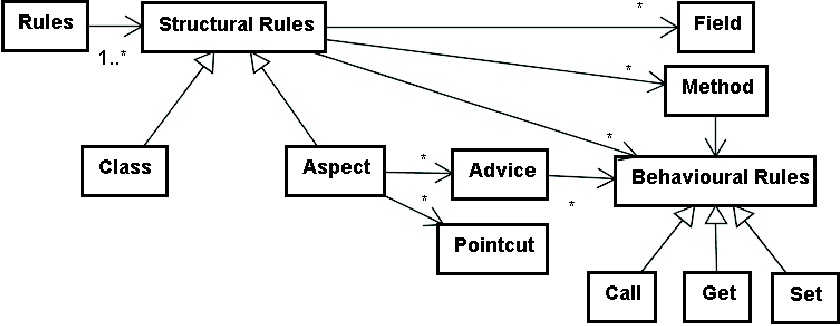
\includegraphics[width=1.0\textwidth]{images/meta-model}\\
%%  \caption{Design Rule Language and Configuration Module Meta-Models}\label{fig:meta-model}
%%  \end{center}
%%\end{figure}
%
%Figure~\ref{fig:meta-model}(a) shows the Design Rules
%specification language meta-model. A rule description is composed
%by one or more structural rules. They are used to define
%structural constraints for classes and aspects. Thus, a class can
%define fields, method signatures and behavioral rules. This
%behavioral rule can be defined within classes and aspects scope or
%within methods and advices. When a behavioral rule is defined
%within the scope of a class or aspect it means that it has to be
%executed at any place, for example, if a rule \emph{call} is used
%within the scope of a class means that the required method must be
%called at least once in any place this class. The
%Figure~\ref{fig:meta-model}(b) depicts the configuration module
%meta-model used to describe a configuration option of the
%specified components by Design Rule. The configuration module
%define which components will follow a particular structural rule
%(\emph{Declaration}) and which parameters (\emph{Parameter}) are
%informed.
%
%For simplicity we do not detail the parametrization mechanism in
%this model. This mechanism can be used to parameterize the method
%signature and fields. For example, we can use the rule
%\emph{set(field)} to allow that a particular field is updated.
%This field could be parameterized and the concrete value would be
%specified by configuration module.
